\title{On a Minkowski-Type Inequality for Multiplicities-II}\label{art06}       
\markright{On a Minkowski-Type Inequality for Multiplicities-II}

\author{By~ B. Teissier}
\markboth{B. Teissier}{On a Minkowski-Type Inequality for Multiplicities-II}

\date{}
\maketitle

\setcounter{page}{407}

\setcounter{pageoriginal}{346}
\textsc{Introduction.}\pageoriginale In the note \cite{art06-keyM.I.}, to which this paper is a sequel, I proved the following Minkowski-type inequality, for multiplicities of primary ideals in a local noetherian Cohen-Macaulay algebra over an algebraically closed field; setting $d = \dim \mathcal{O}$, we have:
\begin{equation*}
e(\mathfrak{n}_1 \cdot \mathfrak{n}_2)^{1/d} \leqslant e(\mathfrak{n}_1)^{1/d} + e(\mathfrak{n}_2)^{1/d} \tag{*}
\end{equation*}
for any two primary ideals $\mathfrak{n}_1$, $\mathfrak{n}_2$ in $\mathcal{O}$, where $e(\mathfrak{n})$ denotes the multiplicity.

In this paper I will prove:

\begin{theorem}\label{art06-thm1}
Let $\mathcal{O}$ be a Cohen-Macaulay normal complex analytic algebra. Then, given two ideals $\mathfrak{n}_1, \mathfrak{n}_2$ of $\mathcal{O}$ which are primary for the maximal ideal, we have the equality
$$
e(\mathfrak{n}_1 \cdot \mathfrak{n}_2)^{1/d} =e(\mathfrak{n}_1)^{1/d}  + e(\mathfrak{n}_2)^{1/d}
$$
if and only if there exist positive integers $a$, $b$ such that 
$$
\overline{\mathfrak{n}^a_1} = \overline{\mathfrak{n}^b_2}
$$
(where the bar means the integral closure of ideals, for the properties of which see {\em \cite{art06-keyC.E.W.}} and {\em \cite{art06-keyL.T.}}).
\end{theorem}

As will be clear from the proof, the conjunction of this result and (*) constitutes a generalization to arbitrary dimension of the classical result asserting the negative definiteness of the intersection matrix of the components of the exceptional divisor of a resolution of singularities of a germ of a normal surface (see \cite{art06-keyDV}, \cite{art06-keyM}, \cite{art06-keyLi}).

This paper also contains two rather different applications of the above result. The first is a lightning proof of a special case of a theorem of Rees (\cite{art06-keyRe}) according to which, given two primary ideals $\mathfrak{n}_1$, $\mathfrak{n}_2$ in an equidimensional ring $\mathcal{O}$ such that $\mathfrak{n}_1 \subset \mathfrak{n}_2$ and $e(\mathfrak{n}_1) = e(\mathfrak{n}_2)$, we have $\overline{\mathfrak{n}_1} = \overline{\mathfrak{n}_2}$.

This\pageoriginale result now plays a rather important role in the study of the geometry of singularities (\cf \cite{art06-keyC.E.W.} and \cite{art06-keyH.L.}) and is also used in the proof of the author's ``principle of specialization of integral dependence'' (\cf \cite{art06-keyD.C.N.} App. I) which is at the source of several results in the theory of equisingularity. The other application is a numerical characterization of those germs of real-analytic maps  $f: (\bfR^2, 0) \to (\bfR^2, 0)$ which are isotopic (in a strong sense) to a germ of a holomorphic map $(\bfC, 0) \to (\bfC, 0)$: they are exactly those maps such that their local topological degree is equal to the square root of the degree of their complexification ($= \dim_\bfR \mathcal{O}_{f^{-1}(0),0} $). This result, which is apparently new, makes use of the algebraic description of the local topological degree, given by Eisenbud and Levine in \cite{art06-keyE.L.}.

\begin{remarks*}
\begin{itemize}
\item[(1)] The equivalence relation: $\mathfrak{n}_1 \sim \mathfrak{n}_2$ if and only if there exist $a$, $b \in \bfN$ such that $\overline{\mathfrak{n}^a_1} = \overline{\mathfrak{n}^b_2}$ has been studied by Samuel in \cite{art06-keySa$_1$}, from a different viewpoint, under  the name ``projective equivalence''.

\item[(2)] The proof of Theorem \ref{art06-thm1} above uses only the Cohen-Macaulay property of $\mathcal{O}$, and the possiblity of resolving singularities of 2-dimensional quotients of $\mathcal{O}$. Indeed it seems to be valid under some mere ``excellence'' assumption on $\mathcal{O}$, (see \cite{art06-keyLi}) and the assumption that $\mathcal{O}$ is Cohen-Macaulay and normal. However, I have in this redaction once again sacrificed generality to geometry, and restricted the presentation to complex analytic geometry to be able to present the ideas in their naivety. In any case, the absence of a base field would indeed make the proofs a lot more cumbersome.
\end{itemize}
\end{remarks*}

\section{A geometric result}\label{art06-sec1}
The essential technical ingredient of the proof of Theorem \ref{art06-thm1} is the following result, in itself rather useful (see \cite{art06-keyT}).

\begin{prop*}
Let $\mathcal{O}$ be a reduced Cohen-Macaulay complex analytic algebra and $\mathfrak{n}$ an ideal of $\mathcal{O}$ primary for the maximal ideal. Set $d = \dim \mathcal{O}$ and let as usual $\mathfrak{n}^{[i]}$ denote an ideal $\mathcal{O}$ generated by $i$ ``sufficiently general'' linear combinations of the elements of a fixed system of generators of $\mathfrak{n}$. Then we have:
\begin{itemize}
\item[{\rm(1)}] $\overline{\mathfrak{n}^{[d]}} = \overline{\mathfrak{n}}$ 

\item[{\rm(2)}] Given\pageoriginale $f \in \mathcal{O}$, $f \in \overline{\mathfrak{n}}$ if and only if 
$$
f \cdot \mathcal{O} / \mathfrak{n}^{[d-1]} \subset \overline{\mathfrak{n} \cdot \mathcal{O}/\mathfrak{n}^{[d-1]}}
$$
with the necessary precision that the meaning of ``sufficiently general'' in the notation $\mathfrak{n}^{[d-1]}$ occurring in (2) depends on $f$, in other words, we have (2) for a Zariski-open dense subset $U_f$ of the space of coefficients of $d-1$ linear combinations of generators of $\mathfrak{n}$, and $U_f$ depends on $f$.
\end{itemize}
\end{prop*}

\begin{proof}
(1), which is due to Samuel \cite{art06-keySa$_2$}, is a consequence of Noether's normalization theorem.

Let us prove (2): let $(W,0)$ be a representative of the germ of complex space corresponding to $\mathcal{O}$, and such that $f$ and $\mathfrak{n}$ are the germs of a globally defined function and ideal on $W$. Let $\pi: \overline{Z} \to W$ be the normalized blowing up of $\mathfrak{n}$ in $W$. It follows from (1) and the results in (\cite{art06-keyH$_1$} Lecture 7, \cite{art06-keyL.T.}) that $\pi$ is also the normalized blowing up of an $\mathfrak{n}^{[d]} = (f_1, \ldots, f_d) \subset \mathfrak{n}$. Let $\pi_0 : Z \to W$ be the blowing up of this $\mathfrak{n}^{[d]}$. Since $\mathcal{O}$ is Cohen-Macaulay, $(f_1, \ldots, f_d)$ is a regular sequence and hence (Lemma 1.9 of \cite{art06-keyH$_2$}) we can describe $\pi_0$ as the restriction of the first projection to the subspace of $W \times \bfP^{d-1}$ defined by the ideal $(f_i T_j - f_j T_i) (1 \leqslant i < j\leqslant d)$, where $(T_1: \ldots : T_d)$ is a system of homogeneous coordinates on $\bfP^{d-1}$.  Let us consider the following diagram:
\[
\xymatrix@R=1.1cm{
& \overline{Z} \ar[d]_n \ar[dr]^\pi & \\
W \times \bfP^{d-1} \ar[dr]_{pr_2} &  Z \ar@{_{(}->}[l] \ar[r]_{\pi_0} \ar[d]^G  & W \\
& \bfP^{d-1} \ar@/^0.6pc/[u]^\sigma & 
}
\]
where\pageoriginale $n$ denotes the normalization map and $\sigma$  is the section of $G = pr_2|Z$ defined by $\sigma (\bfP^{d-1}) = \{0\} \times \bfP^{d-1}$, which is in $Z$ since $\mathfrak{n}^{[d]} \subset \mathfrak{m}$, the maximal ideal of $\mathcal{O}$.

Now we consider $Z {\displaystyle\mathop{\xrightarrow{\curvearrowleft}}^\sigma_G} \bfP^{d-1}$ as a family of germs of curves, which like any family of curves admits a simultaneous normalization (\cite{art06-keyD.C.N.}) over an open-analytic (i.e. complement of a closed analytic subset) dense subset of its parameter space hence, here, over a Zariski open dense subset $U \subset \bfP^{d-1}$. This means that for $p \in U$, the composed map $\overline{G}: \overline{Z} \to Z \to \bfP^{d-1}$ is flat in a neighbourhood of the finite set $n^{-1}(\sigma(p))$, and the multi-germ $((\overline{Z})_p, n^{-1} (\sigma(p)))$ where $(\overline{Z})_p = \overline{G}^{-1} (p)$, is the union of a finite set of germs of non-singular curves, each being the normalization of an irreducible component of the curve $(Z_p, \sigma(p))$, where $Z_p = G^{-1}(p)$. Furthermore since clearly $Z_p$ is ``transversal'' to $\{0\} \times \bfP^{d-1}$ which is set-theoretically the exceptional divisor of $\pi_0$, $(\overline{Z}_p, z_i)$ will be a germ of a non-singular curve transversal to the exceptional divisor $D$ of $\pi$, for $z_i \in n^{-1}(\sigma (p))$. The idea is, that these germs of curves {\em can be used to compute multiplicities along the exceptional divisor $D$ of $\pi$.} Indeed, since $n$ is a finite morphism, each irreducible component $D_i$ of $D$, which is purely of codimension 1 in $\overline{Z}$ by the hauptidealsatz, is mapped surjectively onto $\{0\} \times \bfP^{d-1}$ by $n$. Let us consider the decomposition $D = \bigcup\limits^l_{i=1} D_i$ of $D$ in its irreducible components. Then by the properties of normal spaces, for each given $f \in \mathcal{O}$ we can find a dense open analytic subset $U_i \subset D_i$ such that at each point $z \in U_i$ we have:
\begin{itemize}
\itemsep=0pt
\item[(1)] $(D_z)_{\red}$ is non-singular and coincides with $(D_{i,z})_{\red}$.

\item[(2)] $\overline{Z}$ is non-singular at $z$.

\item[(3)] $f \cdot \mathcal{O}_{\overline{Z}, z}$ defines a subspace having a reduced associated subspace which coincides with $(D_{i,z})_{\red}$, in other words: the strict transform by $\pi$ of $f=0$ is empty near $z$.
\end{itemize}
By diminishing $U$ if necessary, in a way which depends upon $f$, since the $U_i$ do, we can assume:
$$
D_i \cap n^{-1}(\sigma (U)) \subset U_j \qquad (1 \leqslant i \leqslant l).
$$\pageoriginale 
Now for $z\in D_i \cap n^{-1} (\sigma (U))$ we have by (1), (2), (3):
\begin{itemize}
\itemsep=0pt
\item[(i)] $\mathfrak{n} \cdot \mathcal{O}_{\overline{Z}, z} \simeq v^{v_i}_1 \cdot \mathcal{O}_{\overline{Z}, z}$, where 

\item[(ii)] $\mathcal{O}_{\overline{Z}, z} \simeq \bfC \{v_i, \ldots, v_d\} $ by (2).

\item[(iii)] $f \cdot \mathcal{O}_{\overline{Z}, z} \simeq v^{\mu i}_1 \cdot \mathcal{O}_{\overline{Z}, z}$,
\end{itemize}
where $\nu_i$, (\resp $\mu_i$) is the order with which $\mathfrak{n} \cdot \mathcal{O}_{\overline{Z}}$ (\resp $f \circ \pi$) vanishes along $D_i$. This order being locally constant is constant on $U_i$ since $D_i$ is irreducible.

Setting $p = G (n(z))$, certainly one of the components of the curve $(Z_p, \sigma (p))$ has a normalization $((\overline{Z})_p, z)$ which goes through $z$ and is transversal to $D_i$ at $z$. Therefore, since the algebra $\mathcal{O}_{(\overline{Z})_{p},z}$ is isomorphic to $\bfC\{t\}$, and $v_1 \cdot \mathcal{O}_{(\bar{Z})_{p},z}  = a_1 t + a_2 t^2 + \ldots$ with $a_i \in \bfC$, $a_1 \neq 0$, we have, denoting by $v$ the order in $t$ of elements of $\bfC\{ t\}$, i.e. the natural valuation on $\mathcal{O}_{(\overline{Z})_{p},z}$, that 
$$
\begin{cases}
~~ v_i= v (\mathfrak{n} \cdot \mathcal{O}_{(\overline{Z})_{p},z}) \quad (p = G(n(z)), z \in U_i)\\
~~ \mu_i = v(f \cdot \mathcal{O}_{(\overline{Z}_{p},z)}).
\end{cases}
$$

Since the polar locus of a meromorphic function in a normal space is either of codimension 1 or empty, and since by (\cite{art06-keyH$_1$}, \cite{art06-keyL.T.}) $f \in \overline{\mathfrak{n}}$ if and only if $f \cdot \mathcal{O}_{\overline{Z}, z} \subset \mathfrak{n}$, $\mathcal{O}_{\overline{Z},z}$ for all $z \in \pi^{-1}(0)$, we see that $f \in \bar{\mathfrak{n}}$ if and only if $\mu_i \geqslant v_i$ ($(1 \leqslant i \leqslant l)$) and this is {\em equivalent} to the fact that for some $p \in U$, and any irreducible component $Z_{p,i}$ of $Z_p=G^{-1}(p)$, we have $f \cdot \overline{\mathcal{O}_{Z_{p,i}, \sigma(p)}} \subset \mathfrak{n} \cdot \overline{\mathcal{O}_{Z_{p,i}, \sigma(p)}}$ for all $i$, that is: $f \cdot \mathcal{O}_{Z_p, \sigma (p)} \subset \overline{\mathfrak{n}\cdot \mathcal{O}_{Z_p, \sigma (p)}}$
(by the valuative criterion for integral dependance, see \cite{art06-keyH$_1$}, \cite{art06-keyL.T.}). But now it is clear that $Z_p$, $p \in U$ is isomorphic to the curve in $(W,0)$ defined by the $d-1$ equations $\dfrac{f_1}{t_1} = \ldots = \dfrac{f_d}{t_d}$ where $(t_1 : \ldots : t_d)$ are the coordinates of $p$, i.e. the equations $f_i t_{i+1} - f_{i+1} t_i = 0 (1 \leqslant i \leqslant d -1)$, and this means that $(Z_p, \sigma(p))$ is the curve defined by a $\mathfrak{n}^{[d]}$ according to our conventions. This ends the proof of Proposition 1.
\end{proof}

\begin{note*}
The following diagram may perhaps help the reader.
\begin{figure}[H]
\centering 
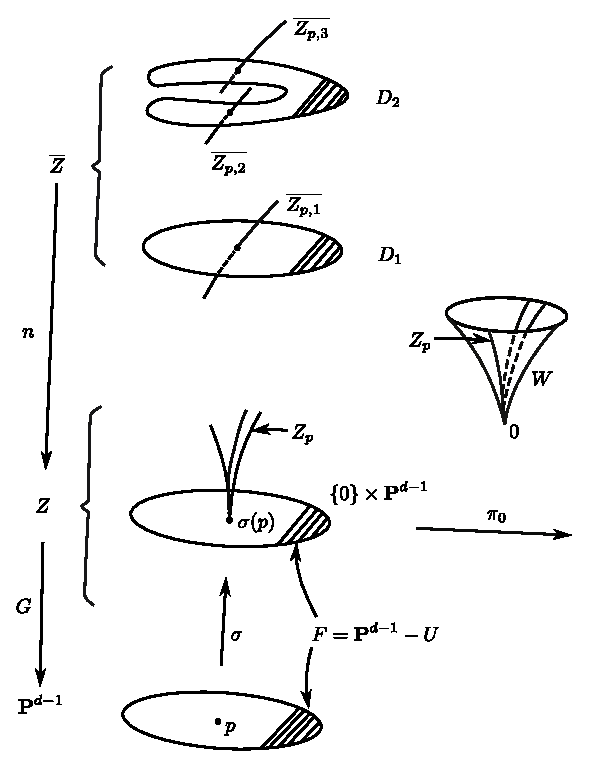
\includegraphics[scale=.9]{fig06-1.eps}
\end{figure}\pageoriginale
\end{note*}

\begin{remark*}
There\pageoriginale is not necessarily a bijection between the irreducible components of $Z_p$, $p \in U$ and those of $D$. What counts is that each $(\mu_i, v_i)$ appears at least once as the valuation of $(\mathfrak{n}, f)$ given by an irreducible component of $Z_p$ and that all these valuations occur in this way. This fact is important in the construction of invariants; see (\cite{art06-keyT}, proof of Theorem \ref{art06-thm2}).
\end{remark*}

\section{Proof of Theorem 1}\label{art06-sec2}
The assertion is obvious when $d = 0, 1$ since $\mathcal{O}$ is then $\bfC$, $\bfC\{t\}$. We therefore assume $d \geqslant 2$. Let us recall from \cite{art06-keyM.I.} that given two primary ideals $\mathfrak{n}_1$ and $\mathfrak{n}_2$ of $\mathcal{O}$, we set
$$
e_i = e \left(\mathfrak{n}^{[i]}_1 + \mathfrak{n}^{[d-i]}_2 \right)
$$
and showed that (*) was a consequence of inequalities
\begin{equation*}
e^d_i \leqslant e^i_d \cdot e^{d-i}_0 \quad (1 \leqslant i \leqslant d)\tag*{[I.2]}
\end{equation*} 
themselves consequences of:
\begin{equation*}
\frac{e_i}{e_{i-1}} \geqslant \frac{e_{i-1}}{e_{i-2}} \quad (2 \leqslant i \leqslant d)
\tag*{[I.3]}
\end{equation*}
All this in view of the equality
\begin{equation*}
e(\mathfrak{n}_1 \cdot \mathfrak{n}_2)  = \sum\limits^d_{i=0} \binom{d}{i} e_i \tag*{[E.1]}
\end{equation*}
of (\cite[Chap. I \S\ 2]{art06-keyC.E.W.}).


The idea being that by induction on $d$ it is enough to prove
$$
\frac{e_d}{e_{d-1}} \geqslant \frac{e_{d-1}}{e_{d-2}}
$$
and that this is in fact a result on surfaces: setting $\mathcal{O} = \mathcal{O} / \mathfrak{n}^{[d-2]}_1$, $\tilde{\mathfrak{n}_i} = \mathfrak{n} \cdot \tilde{\mathcal{O}}$, $i=1$, $2$ we saw, thanks to the Cohen-Macaulay property of $\mathcal{O}$, that $e_d = \tilde{e}_d$, $e_{d-1} = \tilde{e}_1$, $e_{d-2} = \tilde{e}_0$ where $\tilde{e_i} = e(\tilde{\mathfrak{n}}^{[i]}_1 + \tilde{\mathfrak{n}}^{[2-i]}_2)$. We considered a well-chosen resolution of singularities of the germ of surface $S_0$ corresponding to $\tilde{\mathcal{O}}$, say $r : S \to S_0$ such that in particular $\tilde{\mathfrak{n}}^{[2]}_1$, $\tilde{\mathfrak{n}}^{[1]}_1 + \tilde{\mathfrak{n}}^{[1]}_2$, $\tilde{\mathfrak{n}}^{[2]}_2$ and the maximal ideal $\mathfrak{m}$ of $\tilde{\mathcal{O}}$ all become invertible on $S$, $\mathfrak{m} \mathcal{O}_S$ defining a divisor with normal crossings. Then, denoting by $u_k$  (\resp $v_k$) the order of vanishing of $\tilde{\mathfrak{n}}_1 \cdot\mathcal{O}_S$ (\resp $\tilde{\mathfrak{n}}_2 \cdot \mathcal{O}_S$)\pageoriginale along the $k$-th component $E_k$ of $r^{-1}(0)$, we had, using a result of C. P. Ramanujam in \cite{art06-keyR}
\begin{equation*}
\left.
\begin{aligned}
\tilde{e}_2 & = - \sum\limits_{k,k'} \langle E_k, E_{k'} \rangle u_k u_{k'}\\
\tilde{e}_1 & = - \sum\limits_{k,k'} \langle E_k, E_{k'} \rangle u_k v_{k'}\\
\tilde{e}_0 & = - \sum\limits_{k,k'} \langle E_k, E_{k'} \rangle v_k v_{k'}
\end{aligned}
\right|\tag{1}
\end{equation*}
where $\langle, \rangle $ denotes the intersection multiplicities of divisors on $S$ {\em supported in $r^{-1}(0)$}, which is easy to define (see \cite{art06-keyR}).

Now let us remark that, in view of the inequalities mentioned above, if equality holds in (*) then necessarily we have 
$$
\frac{e_d}{e_{d-1}} = \ldots = \frac{e_1}{e_0}.
$$
Let $\dfrac{a}{b}$ denote the common value of these ratios. It follows easily from the results in (\cite{art06-keyC.E.W.} Chap. I \S 2) that if we replace $\mathfrak{n}_1$ by $\mathfrak{n}^a_1$ and $\mathfrak{n}_2$ by $\mathfrak{n}^b_2$, $e_i$  is replaced by $a^i b^{d-i} e_i$. After this substitution we see that the proof of Theorem \ref{art06-thm1} is reduced to proving that if $e_d = e_{d-1} = \ldots = e_0$, then $\overline{\mathfrak{n}}_1 = \overline{\mathfrak{n}}_2$. 

Now by the theorem of Bertini for normality (see \cite{art06-keyF}) we have that $\mathcal{O}/\mathfrak{n}^{[d-2]}_1$ is a normal analytic algebra if $\mathcal{O}$ is so, and then by the classical result (\cite{art06-keyDV}, \cite{art06-keyLi}, \cite{art06-keyM}) the matrix of the $\langle E_k, E_{k'}\rangle $ is negative definite, from which follows immediately in view of (1) that if $\tilde{e}_2 = \tilde{e}_1 =\tilde{e}_0$ we have $u_k = v_k$ for all $k$, hence $\tilde{\mathfrak{n}}_1 \cdot \mathcal{O}_S = \tilde{\mathfrak{n}}_2 \cdot \mathcal{O}_S$ (since $\tilde{\mathfrak{n}}_1 \cdot \mathcal{O}_S$ and $\tilde{\mathfrak{n}}_2 \cdot \mathcal{O}_S$ are invertible on $S$) and from this follows $\overline{\tilde{\mathfrak{n}}_1} = \overline{\tilde{\mathfrak{n}}_2}$ in $\mathcal{O}/\mathfrak{n}^{[d-2]}_1$. Let us now show that $\mathfrak{n}_1 \subset \overline{\mathfrak{n}}_2$ in $\mathcal{O}$: given $f \in \mathfrak{n}_1$, to show that $f \in \overline{\mathfrak{n}}_2$ it is sufficient, in view  of Proposition 1, to show that $f \cdot \mathcal{O} / \mathfrak{n}^{[d-1]}_1\subset \overline{\mathfrak{n}_2\cdot \mathcal{O}/\mathfrak{n}_1^{[d-1]}}$, but certainly a $\mathcal{O}/\mathfrak{n}_1^{[d-1]}$ is a quotient of a $\mathcal{O}/\mathfrak{n}_1^{[d-2]}$ as above, and since $\overline{\tilde{\mathfrak{n}}_1} = \overline{\tilde{\mathfrak{n}}_2}$ we have 
$$
f \cdot \mathcal{O} / \mathfrak{n}^{[d-2]}_1  \subset \overline{\mathfrak{n}_2 \cdot \mathcal{O} / \mathfrak{n}^{[d-2]}_1}
$$
hence\pageoriginale  {\em a fortiori}
$$
f \cdot \mathcal{O} / \mathfrak{n}^{[d-1]}_1 \subset \overline{\mathfrak{n}_2 \cdot \mathcal{O}/ \mathfrak{n}^{[d-1]}_1}. 
$$
This shows that for any $f \in \mathfrak{n}_1$, $f \in \overline{\mathfrak{n}}_2$, i.e., $\mathfrak{n}_1 \subset \overline{\mathfrak{n}}_2$ whence $\overline{\mathfrak{n}}_1 = \overline{\mathfrak{n}}_2$ by symmetry. This proves that if $e(\mathfrak{n}_1 \cdot \mathfrak{n}_2)^{1/d} = e(\mathfrak{n}_1)^{1/d} + e(\mathfrak{n}_2)^{1/d}$  we have $\overline{\mathfrak{n}^a_1} = \overline{\mathfrak{n}^b_2}$. The converse is an immediate consequence of the fact that $e(\mathfrak{n}) = e(\overline{\mathfrak{n}})$ (\cite{art06-keyC.E.W.} Chap. 0) and the remark made about the behaviour of the $e_i$ under the operation $\mathfrak{n} \to \mathfrak{n}^a$. This ends the proof of Theorem \ref{art06-thm1}.

\begin{remark*}
We have seen in the course of the proof that, thanks to (1), when $d =2$, Theorem \ref{art06-thm1} and (*) together follow from the negative definiteness of ($\langle E_k, E_{k'}\rangle $).
\end{remark*}

\section{Applications}\label{art06-sec3}

\subsection{\textsc{First application: the Theorem of Rees} (in a special case).}\label{art06-subsec3.1}

\begin{theorem*}[(Rees)~]
Let $\mathcal{O}$ be a Cohen-Macaulay normal analytic algebra, $\mathfrak{n}_1$ and $\mathfrak{n}_2$ two ideals of $\mathcal{O}$ primary for the maximal ideal and such that $\overline{\mathfrak{n}}_1 \subseteq \overline{\mathfrak{n}}_2$ and $e(\mathfrak{n}_1) = e(\mathfrak{n}_2)$. Then we have $\overline{\mathfrak{n}}_1 =\overline{\mathfrak{n}}_2$. 
\end{theorem*}

\begin{proof}
It is easy to see that for any positive integer $a$, we have $\overline{\mathfrak{n}_1} = \overline{\mathfrak{n}_2} \Leftrightarrow \overline{\mathfrak{n}^a_1} = \overline{\mathfrak{n}^a_2}$ (e.g., use the valuative criterion for integral dependence, \cite{art06-keyH$_1$}, \cite{art06-keyL.T.}). Now let us set $e(\mathfrak{n}_1) = e(\mathfrak{n}_2) = e$. Since for any two primary ideals, $\mathfrak{n} \subseteq \mathfrak{n}'$ implies $e(\mathfrak{n}) \geqslant e (\mathfrak{n}')$, $\mathfrak{n}_1 \subseteq \mathfrak{n}_2$ implies $e(\mathfrak{n}_1 \cdot \mathfrak{n}_2) \geqslant e(\mathfrak{n}^2_2) = 2^d e$. Using (*) now we see that 
$$
2 \cdot e^{1/d} \leqslant e (\mathfrak{n}_1 \cdot \mathfrak{n}_2)^{1/d} \leqslant e^{1/d} + e^{1/d} = 2 \cdot e^{1/d},
$$
hence we have equality, and by Theorem \ref{art06-thm1} there exist $a$, $b \in \bfN$ such that $\overline{\mathfrak{n}^a_1} = \overline{\mathfrak{n}^b_2}$. But we saw that $e(\mathfrak{n}^a) = a^d e (\mathfrak{n})$ and $e (\overline{\mathfrak{n}}) = e(\mathfrak{n})$. Since $e(\mathfrak{n}_1) = e(\mathfrak{n}_2)$, the above equality therefore implies $a=b$, from which the theorem follows.
\end{proof}

\subsection{Second Application}\label{art06-subsec3.2}
Let $f: (\bfR^n, 0) \to (\bfR^n, 0)$ be a germ of a real analytic mapping, described by $f_1 , \ldots, f_n$ in $\bfR \{\underline{x}\} = \bfR\{ x_1,\ldots, x_n\}$ and such that $Q (f) = \mathcal{O}_{f-1_{(0),0}} = \bfR \{\underline{x}\}/(f_1, \ldots, f_n)$ is  a finite dimensional\pageoriginale vector space over $\bfR$. Set $q =\dim_\bfR Q (f); q$ is also the topological degree of the complexified map $f^\bfC: (\bfC^n, 0) \to (\bfC^n,0)$. It was proved in \cite{art06-keyE.L.} that the topological degree deg $f$ of $f$ satisfies
$$
|\deg f| \leqslant q^{1-1/n}
$$
and this inequality was proved as follows: first one proved that $|\deg f| \leqslant e(\mathfrak{n}^{[n-1]} + \mathfrak{m}^{[1]})$ where $\mathfrak{n}$ is the ideal generated by $(f_1, \ldots, f_n)$ in $\bfC \{\underline{x}\}$ and $\mathfrak{m}$ is the maximal ideal, then one used the inequality [1.2] from \cite{art06-keyM.I.} quoted above to show that 
$$
e (\mathfrak{n}^{[n-1]} + \mathfrak{m}^{[1]}) \leqslant e (\mathfrak{n})^{1-1/n} = q^{1-1/n}.
$$

Let us consider the special case $n =2$. We have $|\deg f| \leqslant q^{1/2}$ and there is at least one case where we have equality: let $f$ be a holomorphic map $(\bfC, 0) \to (\bfC, 0)$ given by $z \mapsto z^k$. Setting $z = x_1 + ix_2$ we see that the components of $f$, $f_1 (x_1, x_2)$ and $f_2(x_1, x_2)$ are homogeneous  polynomials of degree $k$. From the additivity of intersection multiplicities follows that in this case $q = k^2$. By writing $z = \rho \cdot e^{i\theta}$ we see that all the zeroes of $f_1$ and $f_2$ are real, and the $k$ lines in $\bfR^2$ where $f_1$ vanishes {\em alternate} with the $k$ lines where $f_2$ vanishes, being obtained from them by a rotation of $\pi/2k$. Furthermore each of the sets of lines divides $\bfR^2$ in $2k$ sectors. One readily checks that $\re z^k =t$, $\Iim z^k=0$ is a regular fibre of $f$, at each point of which $f$ preserves the orientation, and which contains $k$ points, since $\re z^k =t$ defines a curve in every second sector among those defined by $\re z^k =0$, which is asymptotic to the walls of this sector and meets the lines $\Iim z^k =0$ transversally. We  remark that the fact that $f$ is orientation preserving comes from the following property of $f_2 = \Iim z^k$, $f_1 = \re z^k$:
\begin{itemize}
\item[(OR)] In each sector where $f_1 > 0$, the sign of $f_2$ changes  from $-$ to $+$ as we cross the line $f_2=0$ circulating in the trigonometric direction (counterclockwise).
\end{itemize}

Having seen this, we have no difficulty in proving 

\begin{lem}\label{art06-lem1}
Let $f: (\bfR^2, 0) \to (\bfR^2, 0)$ be given by two homogeneous polynomials $f_1$, $f_2$ of the same degree $k$. Then we have $\deg f = k $ if, and only if,\pageoriginale $f_1$ and $f_2$ both have all their roots real, these roots alternate and the condition (OR) is satisfied.
\end{lem}

Indeed, if they do not both have all their roots real, we can find a regular fibre with less than $k$ points, hence $|\deg f| < k$. If they do not alternate, then we can find two points in a fibre with $k$ points, where the orientation is not the same, hence again $|\deg f| < k$ and finally if the first two conditions are satisfied we have $\deg f = \pm k$, and condition (OR) implies $\deg f - k$ (and conversely). We now prove:

\begin{lem}\label{art06-lem2}
Let $f = (f_1, f_2)$ and $f' = (f'_1, f'_2)$ {\em  be two mapping satisfying}  the condition of Lemma \ref{art06-lem1}. Then there is a 1-parameter family $(f_t)_{t \in [0,1]}$ of mappings, all satisfying the condition of Lemma \ref{art06-lem1}, such that $f_0 \simeq f$ and $f_1 \simeq f'$.
\end{lem}
 
\begin{proof}
After a suitable choice of coordinates, we can write (up to the isomorphism corresponding to a constant factor)
$$
f_1 = \prod\limits^k_{i=1} (x_1 - \alpha_i x_2) \quad f_2 = \prod\limits^k_{i=1} (x_1 - \beta_i x_2) \quad \alpha_i, \beta_i \in \bfR 
$$
with $\alpha_1 < \beta_1 < \alpha_2 < \ldots < \alpha_k < \beta_k$, and similarly
$$
f'_1 = \prod\limits^k_{s =1} (x_1 - \alpha'_i x_2), \quad f'_2 =\prod\limits^k_{i=1} (x_1 -\beta'_i x_2)
$$
with $\alpha'_1, < \beta'_1 < \alpha'_2 < \ldots < \alpha'_k < \beta_k'$.

Then  the family given by
\begin{align*}
f_{t,1} & = \prod\limits^k_{i=1} (x_1 - (t\alpha'_i + (1-t)\alpha_i) x_2)\\
f_{t,2} & = \prod\limits^k_{i=1} (x_1 - (t\beta'_i + (1-t) \beta_i)x_2)
\end{align*}
for $0 \leqslant t \leqslant 1$, obviously gives the answer.
\end{proof}

\begin{theorem}\label{art06-thm2}
Let $f: (\bfR^2,0) \to (\bfR^2, 0)$ be a germ of a real-analytic mapping with algebraic degree $q(q = \dim_\bfR \mathcal{O}_{f-1^{(0),0}})$. Then $f$ can be continuously deformed, with degree and algebraic degree both constant, to a holomorphic mapping $(\bfC,0) \to (\bfC,0)$ if and only if $\deg f = q^{1/2}$.
\end{theorem}

\begin{proof}
The condition\pageoriginale is obviously necessary, after what we have just seen. Let us prove it sufficient. From what we saw above, the equality $\deg f = q^{1/2}$ implies $e(\mathfrak{n}^{[1]} + \mathfrak{m}^{[1]}) = e(\mathfrak{n})^{1/2}$ which, since $e(\mathfrak{m}) =1$, and in view of the equality ($E$. 1) quoted in \S \ref{art06-sec2}, gives $e(\mathfrak{n} \cdot \mathfrak{m})^{1/2} = e(\mathfrak{n})^{1/2}+ e(\mathfrak{m})^{1/2}$. From Theorem \ref{art06-thm1} we deduce the existence of integers $a$, $b$ such that $\overline{\mathfrak{n}^a} = \overline{\mathfrak{m}^b}$ and from the properties of multiplicities we deduce that in fact we must have $\overline{n} = \mathfrak{m}^k$ in $\bfC \{x_1, x_2\}$, where $k = q^{1/2} = \deg f$. We are going to show that this implies that the components $f_1$, $f_2$ of $f$ can be taken (up to isotopy) to be homogeneous polynomials of degree $k$. Let $\mathfrak{n}'$ be the ideal in $\bfC\{x_1, x_2\}$ generated by those among $(f_1, f_2)$ which are in $\mathfrak{m}^k - \mathfrak{m}^{k+1}$: we have $\mathfrak{n}' \subset \mathfrak{n} \subset \mathfrak{n}' + \mathfrak{m}^{k+1}$ hence, since $\overline{\mathfrak{n}} = \mathfrak{m}^k$, we have $\overline{\mathfrak{n}' + \mathfrak{m} \cdot \mathfrak{m}^k} = \mathfrak{m}^k$ which by the integral Nakayama Lemma (\cite{art06-keyC.E.W.} Chap. 11, 2.4)  implies $\overline{\mathfrak{n}'} = \mathfrak{m}^k$, which in turn implies that $\mathfrak{n}'$ is generated by at least two elements, whence $\mathfrak{n}' =\mathfrak{n}$. Now we know $f_i \in \mathfrak{m}^k - \mathfrak{m}^{k+1}$, $i =1,2$. We can set 
\begin{align*}
f_1 & = P_k + P_{k+1} + \ldots \\
f_2 & = Q_k + Q_{k+1} + \ldots 
\end{align*}
where $P_i$ (or $Q_i$) is an homogeneous polynomial of degree $i$ in $x_1$ and $x_2$. We know furthermore that since $\mathfrak{n}' = (P_k, Q_k)$ has at its integral closure $\mathfrak{m}^k$, $\dim_\bfR \bfR \{x_1, x_2\} / (P_k, Q_k) = \dim_\bfR \bfR \{x_1, x_2\}/ (f_1, f_2) = q$. Consider the family of functions
\begin{align*}
f_{1,t} & = P_k + t P_{k+1} + \ldots + t^l P_{k+l} + \ldots \\
f_{2,t} & = Q_k + t Q_{k+1} + \ldots + t^l Q_{k+l} + \ldots 
\end{align*} 
the family of ideals $\mathscr{F}_t = (f_{1,t}, f_{2,t}) \cdot \bfR \{x_1, x_2\}$ and the family of algebras $Q_t = \bfR \{x_1, x_2\} / \mathscr{F}_t$. For any $t \neq 0$, $Q_t$ is isomorphic to $Q(f)$ as an $\bfR$-algebra (change $x_i$ to $tx_i$ in $f$, and divide by $t^k$), and $Q_0= \bfR \{x_1, x_2\} / (P_k, Q_k)$.

We now use the main result of \cite{art06-keyE.L.}: all the $Q_t$ are isomorphic as vector spaces; choosing a linear form $l: Q_0\to \bfR$ such that $l(J_0)>0$, where $J_0$ is the Jacobian determinant of $(P_k, Q_k)$, we can extend $l$ to $Q_t$ and denoting by $J_t$ the Jacobian determinant of $(f_{1,t},f_{2,t})$, we get $l(J_t)>0$\pageoriginale  for $t$ sufficiently small. According to Theorem 1.2 of \cite{art06-keyE.L.}, we have:
\begin{enumerate}
\item[(1)] the bilinear form on $Q_t$ defined by $\langle p, q\rangle  =l(p\cdot q)$ is non-singular for all sufficiently small $t$, therefore its signature is independent of $t$ near $t =0$.

\item[(2)] This signature is equal to $\deg f$ for $t \neq 0$ and to the degree of the $\map f_0 : (\bfR^2, 0) \to (\bfR^2 , 0)$ defined by $(P_k, Q_k)$ for $t =0$.
\end{enumerate}

Hence $\deg f_0 = k = q^{1/2}$ and Theorem \ref{art06-thm2} now follows easily from Lemmas \ref{art06-lem1} and \ref{art06-lem2}. 
\end{proof}

\begin{remarks*}
\item[(1)] The key point is to check that the assumption $\deg f = q^{1/2}$ implies that the tangent cones at 0 of $f_1 = 0$ and $f_2 = 0$ have the same degree, and no common component. This is what Theorem \ref{art06-thm1} does for us in the above proof.

\item[(2)] Theorem \ref{art06-thm2} above is valid also for $C^\infty$ maps $f: (\bfR^2, 0) \to (\bfR^2, 0)$ such that $\dim \mathscr{E}_2 / (f_1, f_2) < \infty$ where $\mathscr{E}_2$ is the ring of germs of $C^\infty$ function on $(\bfR^2, 0)$, since the finiteness assumption implies that in those problems we have finite determinacy (see \cite{art06-keyE.L.}).

\item[(3)] It is an interesting problem to find invariants of algebras of the form $\bfR \{x_1, \ldots, x_n\} / (f_1, \ldots, f_n)$ of finite dimension over $\bfR$ which allow one to determine when two such algebras (or the corresponding germs of mappings $(\bfR^n, 0) \to (\bfR^n, 0)$) can be continuously deformed into one another with constant dimension of the algebras (i.e. algebraic degree) and degree. 
\end{remarks*}

\begin{thebibliography}{99}
\bibitem[C.E.W.]{art06-keyC.E.W.} B. Teissier, Cycles \'evanescents, sections planes et conditions de Whitney, {\em Ast\'erique } No 7-8 (1973), 285-362, Soc. Math Fr.

\bibitem[D.C.N.]{art06-keyD.C.N.} B. Teissier, {\em Sur diverses conditions num\'eriques d'\'equisingularit\'e pour les familles de courbes (et un principe de sp\'ecialisation de\pageoriginale la d\'ependance int\'egrale),} Centre de Maths. de l'Ecole Polytechnique, F 91128 Palaiseau. See also: S\'eminaire Demazure-Pinkham-Teissier sur les Singularit\'es des surfaces 1976-1977 (to appear).

\bibitem[DV]{art06-keyDV} P. Du Val, On isolated singularities of surfaces which do not affect the condition of adjunction, I, {\em Proc. Cambridge Phil. Soc. }  30 (1934), 453-459.


\bibitem[E.L.]{art06-keyE.L.} D. Eisenbud and H. Levine, An algebraic formula for the degree of a $C^\infty$ map-germ, {\em Ann. of Maths.} 106, 1 (1977).

\bibitem[F]{art06-keyF} H. Flenner, Die S\"atze von Bertini f\"ur lokale Ringe, {\em Math. Ann. 229 (1977), 97-111.}

\bibitem[H$_1$]{art06-keyH$_1$} H. Hironaka, {\em Introduction to the theory of infinitely near singular points, } Memorias de Matematica del Instituto Jorge Juan, Serrano 123, Madrid 6, Spain (1974).

\bibitem[H$_2$]{art06-keyH$_2$} H. Hironaka, Smoothing of algebraic cycles of small dimension, {\em Amer. J. Maths.} Vol. 90, No 1 (1968).

\bibitem[H.L.]{art06-keyH.L.} J. P. G. Henry et Le Dung Trang, {\em Limites d'espaces tangents}, Springer Lecture Notes in Maths. No 482 (1975), 252-265.


\bibitem[L.T.]{art06-keyL.T.} M. Lejeune-Jalabert et B. Teissier, S\'eminaire 1973-74 {\em ``Cl\^oture int\'egrale des id\'eaux et \'equisingularit\'e'',} disponible \`a l'Institut Fourier, Fac. des Sciences 38402 St Martin d'H\'eres.

\bibitem[Li]{art06-keyLi} J. Lipman, Rational singularities, {\em Publ. Math. I.H.E.S.} No 36 (1968), 195-279.

\bibitem[M.I.]{art06-keyM.I.} B. Teissier, Sur une in\'egalit\'e \`a la Minkowski pour les multiplicit\'es, Appendix to [E.L.].

\bibitem[M]{art06-keyM} D. Mumford, The topology of normal singularities of an algebraic surface, {\em Publ. Math. I.H.E.S. No 9 (1961).}

\bibitem[R]{art06-keyR} C. P. Ramanujam, On a geometric interpretation of multiplicity, {\em Inventiones Math.} 22 (1973), 63-67.

\bibitem[Re]{art06-keyRe} D. Rees, A-transforms of local rings, {\em Proc. Cambridge Phil. Soc. } Vol. 57 (1961), 8-17.

\bibitem[Sa$_1$]{art06-keySa$_1$} P. Samuel,\pageoriginale Some asymptotic properties of powers of ideals, {\em Ann. of Maths. } Vol. 56 No 1 (1952), 11-21.

\bibitem[Sa$_2$]{art06-keySa$_2$} P. Samuel, La notion de multiplicit\'e en alg\'ebre et g\'eom\'etrie alg\`ebrique, {\em J. Maths. Pures et Appl. } 30 (1951), 159-274.

\bibitem[T]{art06-keyT} B. Teissier, Invariants polaires I. Invariants polaires des hypersurfaces, {\em Inventiones Math.} 40 (1977), 267-292.

\end{thebibliography}
